\documentclass{beamer}
\usetheme{Boadilla}

\usepackage{amsmath, amssymb, physics}
\usepackage{tikz}
\usetikzlibrary{arrows.meta, shapes, positioning}

\title[0-D SRM Model]{Zero-Dimensional Solid Rocket Motor Internal Ballistics}
\subtitle{Mass, Energy, and Pressure Dynamics for AP/HTPB Composite Propellants}
\author{Prepared for: Graduate Propulsion Systems Design}
\date{}

\begin{document}

%==================================================================
\frame{\titlepage}
%==================================================================

%==================================================================
\begin{frame}{Control Volume and Basic Assumptions}
    \begin{itemize}
        \item Control volume = gas inside the combustion chamber.
        \item Gas assumed perfectly mixed and spatially uniform.
        \item Ideal gas: $pV = mRT$.
        \item Sources:
        \begin{itemize}
            \item Propellant–generated mass $\dot m_b$
            \item Igniter mass $\dot m_{\text{ign}}$
            \item Heat release from combustion $\dot Q_{\text{comb}}$
        \end{itemize}
        \item Sinks:
        \begin{itemize}
            \item Nozzle mass flow $\dot m_e$
            \item Wall heat losses $\dot Q_{\text{wall}}$
        \end{itemize}
    \end{itemize}

    \centering
    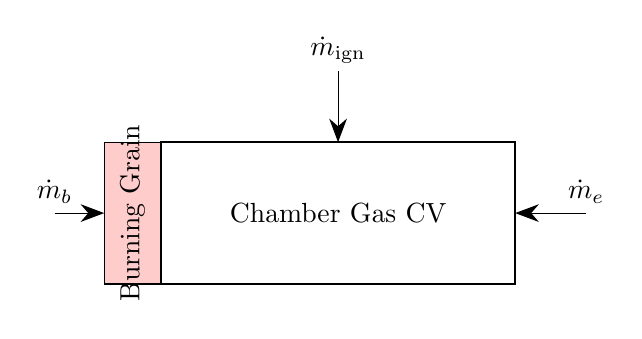
\begin{tikzpicture}[scale=0.9]
        % Chamber
        \draw[thick] (0,0) rectangle (5,2);
        \node at (2.5,1) {Chamber Gas CV};
        % Burn surface
        \draw[fill=red!20] (-0.8,0) rectangle (0,2);
        \node[rotate=90] at (-0.4,1) {Burning Grain};
        % Arrows
        \draw[-{Stealth[length=3mm]}] (-1.5,1) -- (-0.8,1);
        \node at (-1.5,1.3) {$\dot m_b$};
        \draw[-{Stealth[length=3mm]}] (6,1) -- (5,1);
        \node at (6,1.3) {$\dot m_e$};
        \draw[-{Stealth[length=3mm]}] (2.5,3) -- (2.5,2);
        \node at (2.5,3.3) {$\dot m_{\text{ign}}$};
    \end{tikzpicture}
\end{frame}
%==================================================================

%==================================================================
\begin{frame}{Mass Balance}
    Total gas mass:
    $$
        \frac{dm}{dt} = \dot m_b + \dot m_{\text{ign}} - \dot m_e
    $$
    Propellant mass generation:
    $$
        \dot m_b = \rho_p\, r_b\, A_b(s)
    $$
    Saint–Robert burn law:
    $$
        r_b = f_{\text{ign}}(t)\,a\,p^n
    $$
    Ignition ramp:
    $$
        f_{\text{ign}}(t) = 1 - \exp\!\left(-\frac{t - t_{\text{ign,start}}}{\tau_{\text{ign}}}\right)
    $$
    Choked nozzle mass flow:
    $$
        \dot m_e = C_d A_t p \sqrt{\frac{\gamma}{RT}}\left(\frac{2}{\gamma+1}\right)^{\frac{\gamma+1}{2(\gamma-1)}}
    $$
\end{frame}
%==================================================================

%==================================================================
\begin{frame}{Energy Balance with Heat Release}
    Internal energy:
    $$
        U = m c_v T
    $$
    Full unsteady first law:
    $$
        \frac{d}{dt}(m c_v T)= \dot m_b h_b + \dot m_{\text{ign}} h_{\text{ign}} - \dot m_e h_e - p\frac{dV}{dt} + \dot Q_{\text{wall}} + \dot Q_{\text{comb}}
    $$
    Combustion heat release:
    $$
        \dot Q_{\text{comb}} = \dot m_b \Delta h_c
    $$
    Total heat term:
    $$
        \dot Q = \dot Q_{\text{wall}} + \dot Q_{\text{comb}} + \dot Q_{\text{ign}}.
    $$
\end{frame}
%==================================================================

%==================================================================
\begin{frame}{Deriving $\frac{dp}{dt}$ (Step 1)}
    Start with:
    $$
        U = m c_v T
    $$
    $$
        \frac{d}{dt}(m c_v T) = \dot m_b h_b + \dot m_{\text{ign}} h_{\text{ign}} - \dot m_e h_e - p\frac{dV}{dt} + \dot Q
    $$
    Assume:
    $$
        h_b \approx h_e \approx c_p T, \qquad h_{\text{ign}} \approx c_p T_{\text{ign}}
    $$
    Left side:
    $$
        \frac{d}{dt}(mc_vT)= c_v\left(m\frac{dT}{dt} + T\frac{dm}{dt}\right)
    $$
    Right side becomes:
    $$
        c_p T\frac{dm}{dt} - p\frac{dV}{dt} + \dot Q
    $$
    Use mass balance:
    $$
        \frac{dm}{dt} = \dot m_b + \dot m_{\text{ign}} - \dot m_e
    $$
\end{frame}
%==================================================================

%==================================================================
\begin{frame}{Deriving $\frac{dp}{dt}$ (Step 2)}
    Rearrange:
    $$
        c_v m\frac{dT}{dt}= (c_p-c_v)T\frac{dm}{dt} - p\frac{dV}{dt} + \dot Q
    $$
    Use $c_p-c_v = R$:
    $$
        \frac{dT}{dt}= \frac{R T\frac{dm}{dt} - p\frac{dV}{dt} + \dot Q}{c_v m}
    $$
    Differentiate ideal gas:
    $$
        pV = mRT
    $$
    $$
        \frac{dp}{dt}V + p\frac{dV}{dt}= R\left(T\frac{dm}{dt} + m\frac{dT}{dt}\right)
    $$
    Substitute above $dT/dt$ expression.
\end{frame}
%==================================================================

%==================================================================
\begin{frame}{Deriving $\frac{dp}{dt}$ (Step 3)}
    Compute:
    $$
        R\left(T\frac{dm}{dt} + m\frac{dT}{dt}\right)= R T\frac{dm}{dt}+ \frac{R}{c_v}\left(R T\frac{dm}{dt} - p\frac{dV}{dt} + \dot Q\right)
    $$
    Use $\gamma = \frac{c_p}{c_v}$ and $\frac{R}{c_v}=\gamma-1$:
    $$
        = \gamma R T\frac{dm}{dt} - (\gamma-1)p\frac{dV}{dt}+ (\gamma-1)\dot Q
    $$
    Insert into:
    $$
        \frac{dp}{dt}V + p\frac{dV}{dt}= R\left(T\frac{dm}{dt} + m\frac{dT}{dt}\right)
    $$
    Thus:
    $$
        \frac{dp}{dt}V= \gamma RT\frac{dm}{dt} - \gamma p\frac{dV}{dt}+ (\gamma-1)\dot Q
    $$
\end{frame}
%==================================================================

%==================================================================
\begin{frame}{Deriving $\frac{dp}{dt}$ (Final Form)}
    Divide by $V$:
    $$
        \frac{dp}{dt}= \frac{\gamma RT}{V}\frac{dm}{dt} - \frac{\gamma p}{V}\frac{dV}{dt}+ \frac{\gamma-1}{V}\dot Q
    $$
    Use ideal gas $pV=mRT$:
    $$
        \frac{RT}{V}=\frac{p}{m}
    $$
    Therefore:
    $$
        \boxed{\frac{dp}{dt}= \gamma p\left[\frac{1}{m}\frac{dm}{dt}- \frac{1}{V}\frac{dV}{dt}\right]+ \frac{\gamma-1}{V}\dot Q}
    $$
    This is the unsteady chamber pressure equation used in 0-D SRM modeling.
\end{frame}
%==================================================================

%==================================================================
\begin{frame}{Volume Evolution and Web Regression}
    Web regression:
    $$
        \frac{ds}{dt} = r_b = f_{\text{ign}}(t)\,a\,p^n
    $$
    Grain geometry tables:
    $$
        A_b(s), \qquad V(s), \qquad \frac{dV}{ds}(s)
    $$
    Chamber volume evolution:
    $$
        \frac{dV}{dt} = \frac{dV}{ds}(s)\,\frac{ds}{dt}
    $$
    \centering
    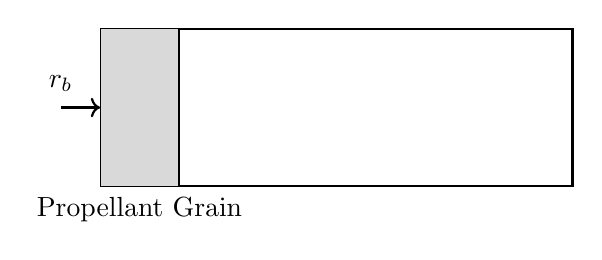
\begin{tikzpicture}
        \draw[thick] (0,0) rectangle (5,2);
        \draw[fill=gray!30] (-1,0) rectangle (0,2);
        \draw[thick,->] (-1.5,1) -- (-1,1);
        \node at (-1.5,1.3) {$r_b$};
        \node at (-0.5,-0.3) {Propellant Grain};
    \end{tikzpicture}
\end{frame}
%==================================================================

%==================================================================
\begin{frame}{Nozzle Throat Erosion}
    Throat area:
    $$
        A_t = \pi r_t^2
    $$
    Erosion model:
    $$
        \frac{dr_t}{dt} = k_{\text{eros}} |\dot m_e|
    $$
    \centering
    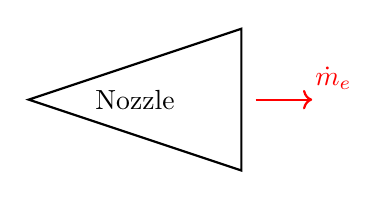
\begin{tikzpicture}[scale=0.9]
        \draw[thick] (0,0) -- (3,1) -- (3,-1) -- cycle;
        \node at (1.5,0) {Nozzle};
        \draw[red,thick,->] (3.2,0) -- (4,0);
        \node[red] at (4.3,0.3) {$\dot m_e$};
    \end{tikzpicture}
\end{frame}
%==================================================================

%==================================================================
\begin{frame}{Final Pressure Equation (SRM Form)}
    With the SRM source terms:
    $$
        \frac{dm}{dt} = \dot m_b + \dot m_{\text{ign}} - \dot m_e,\qquad \frac{dV}{dt} = \frac{dV}{ds}(s)\frac{ds}{dt},
    $$
    the chamber pressure ODE is:
    $$
        \boxed{\frac{dp}{dt}= \gamma p\left[\frac{\dot m_b + \dot m_{\text{ign}} - \dot m_e}{m}- \frac{1}{V}\frac{dV}{dt}\right]+ \frac{\gamma - 1}{V}\dot Q}
    $$
\end{frame}
%==================================================================

%==================================================================
\begin{frame}{Final ODE System}
    State vector:
    $$
        y(t)=\begin{bmatrix}p(t)\\[4pt]m(t)\\[4pt]s(t)\\[4pt]r_t(t)\end{bmatrix}
    $$
    ODEs:
    $$
        \frac{dp}{dt}= \gamma p\!\left[\frac{\dot m_b + \dot m_{\text{ign}} - \dot m_e}{m}- \frac{1}{V}\frac{dV}{dt}\right]+ \frac{\gamma - 1}{V}\dot Q
    $$
    $$
        \frac{dm}{dt} = \dot m_b + \dot m_{\text{ign}} - \dot m_e
    $$
    $$
        \frac{ds}{dt} = f_{\text{ign}}(t)\,a\,p^n
    $$
    $$
        \frac{dr_t}{dt} = k_{\text{eros}}|\dot m_e|
    $$
\end{frame}
%==================================================================

%==================================================================
\begin{frame}{Assumptions \& Limitations of the 0-D SRM Model}
    	extbf{Major assumptions:}
    \begin{itemize}
        \item Chamber gas is \textbf{perfectly mixed} (no spatial gradients).
        \item Propellant gases instantaneously reach chamber temperature.
        \item Ideal-gas thermodynamics: $pV=mRT$.
        \item Quasi-steady Saint–Robert burn law: $r_b = a p^n$.
        \item Choked nozzle flow with fixed $C_d$.
        \item Lumped heat loss: $\dot Q_{\text{wall}} = -h_wA_w(T-T_w)$.
        \item Grain geometry encoded through tables $A_b(s)$ and $V(s)$.
    \end{itemize}
    	extbf{Limitations:}
    \begin{itemize}
        \item Cannot predict combustion instabilities or pressure oscillations.
        \item No axial or transverse wave dynamics (1-D/3-D neglected).
        \item No local flame chemistry or finite-rate kinetics.
        \item No particle dynamics (Al droplets, slag accumulation).
        \item No two-phase flow in nozzle.
        \item No detailed heat transfer to insulation or case.
    \end{itemize}
    \centering
    	extit{Useful for system-level design and grain optimization, but not for high-fidelity stability or transient ignition modeling.}
\end{frame}
%==================================================================

\end{document}